\documentclass[12pt,twoside,a4paper]{article}

% Set the margin
\usepackage[margin=2.05cm]{geometry}

% Use the AMS symbols package for special fonts such as mathbb
\usepackage{amssymb}

% Use the calc package for infix arithmetic
\usepackage{calc}

% Use BibTeX for bibliography management, use the hyperref package to include URLs in the entries
\usepackage{cite}
\usepackage{url}

% Define macros for correct spacing after abbreviations, source: http://tex.stackexchange.com/a/15017
\usepackage{xspace}
\newcommand*{\eg}{e.g.\@\xspace}
\newcommand*{\ie}{i.e.\@\xspace}
\newcommand*{\iid}{i.i.d.\@\xspace}

\makeatletter
\newcommand*{\etc}{%
    \@ifnextchar{.}%
        {etc}%
        {etc.\@\xspace}%
}
\makeatother

% Use the tikz package for drawing
\usepackage{tikz}

% Define a new tikz style for drawings left-closed intervals: [i], notice that the heads are centred exactly on the start and end coordinates of the line
\usetikzlibrary{decorations.markings}
\tikzset{
    i/.style={
        shorten >=#1,
        decoration={
            markings,
            mark={ at position 0 with {\filldraw[solid] circle [radius=#1];} },
            mark={ at position 1 with {\draw[solid] circle [radius=#1];} }
        },
        postaction=decorate
    },
    i/.default=1.5pt
}

% Define a macro for drawing an interval, the arguments are always:
%	(#1,#2)	- start position
%	(0,#3)	- length vector
%	(#4,#5)	- beginning and end of the interval, normalised between 0 and 1
%	#6		- line style
%	#7		- position of the label ("left" or "right") if the interval is labelled
\newcommand{\interval}[6] {
	\draw[#6] [i] (#1,#2+#4*#3) -- (#1,#2+#5*#3);
}

\newcommand{\intervalTopLabel}[7] {
	\interval{#1}{#2}{#3}{#4}{#5}{#6}
	\node[#7] at (#1,#2+#5*#3) {\footnotesize #5};
}

\newcommand{\intervalBottomLabel}[7] {
	\interval{#1}{#2}{#3}{#4}{#5}{#6}
	\node[#7] at (#1,#2+#4*#3) {\footnotesize #4};
}

\newcommand{\intervalBothLabels}[7] {
	\intervalBottomLabel{#1}{#2}{#3}{#4}{#5}{#6}{#7}
	\node[#7] at (#1,#2+#5*#3) {\footnotesize #5};
}

\begin{document}

\title{Hiding Secrets in Plain Text \\ {\large \textbf{4th year project technical milestone report}}}
\author{by Konrad Komorowski \\ {supervised by Dr.~Jossy Sayir} \\ {\normalsize \textbf{CUED Signal Processing and Communications Laboratory}}}
\date{January 16, 2014}
\maketitle

\begin{abstract}
The objective of the project is to create a secure steganographic communications system. The system should translate any message into an innocuous stream of English text secured by a private key. Only the knowledge of the key should allow to detect and retrieve the message. A working proof of concept of the system, which does not yet implement secrecy, has been created. The next main areas of focus will be implementation of secrecy and improvement of the language models used in the generation of output text.
\end{abstract}

\section{Aim}
\label{sec:aim}

The aim of the project is to create a communications system that will allow to broadcast a secret message enciphered with a private key as a paragraph of pseudo-randomly generated English text. The system should also translate this paragraph back into the original message using the same key. The sentences should appear to be randomly drawn from the set of all possible English sentences -- in other words will seem innocuous for an enemy monitoring communications between two parties. The introduction of a private key means that the secrecy of the message does not rely on the enemy's unfamiliarity with the system, but on a private piece of information exchanged between the two parties.

\section{Overview of steganography}
\label{sec:steganography_overview}

The project falls in the field of \emph{steganography}, which can be defined as follows:

\begin{quote} Steganography is the art and science of encoding hidden messages in such a way that no one, apart from the sender and intended recipient, suspects the existence of the message. \cite{wiki:steganography} \end{quote}

An example stegosystem providing some \emph{innocuousness} and \emph{secrecy} can be constructed in the following way:

\begin{quote} A message, the \emph{plaintext}, may be first encrypted by traditional means, producing a \emph{ciphertext}. Then, an innocuous \emph{covertext} is modified in some way so as to contain the \emph{ciphertext}, resulting in the \emph{stegotext}. \cite{wiki:steganography} \end{quote}

There are various ways in which ciphertext may be embedded in covertext:
\emph{a)}~by breaking the lines of covertext in such a way that the first words of every line form ciphertext -- this works if stegotext is not reformatted in transmission;
\emph{b)}~by replacing standard characters with their redundant Unicode lookalikes according to ciphertext  -- this works if stegotext is transmitted using Unicode;
\emph{c)}~by modifying noise in covertext according to ciphertext -- this works if a rasterised version of stegotext is transmitted \emph{exactly} (\ie digitally, not in print).

The methods outlined above provide only some degree of innocuousness. They largely rely on the enemy's unfamiliarity with the system and may be detected using statistical tests, \eg identifying unusual distributions of Unicode characters or image noise.

\section{The interval algorithm}
\label{sec:interval_algorithm}

The interval algorithm \cite{hanhoshi1997} provides a means of sampling from an arbitrary stochastic process (target) given an input sequence from a different arbitrary stochastic process (source). The algorithm is very similar to arithmetic coding -- it also uses successive refinements of the $[0,1)$ interval to map sequences.

The sequence mapping algorithm starts by mapping the empty sequence $[~]$ to the interval $[0,1)$. For any sequence, its interval is partitioned into subintervals corresponding to the sequence extended by a single term. The size of each interval is chosen to be proportional to the probability of the last term occurring given the preceding sequence. The order of the subintervals does not matter, but needs to be consistent if reverse mapping from an interval to a sequence is to be performed. By the chain rule of probability, the size of the resulting interval is equal to the probability of observing its sequence. Consequently, only sequences of non-zero probability can be mapped. For a more detailed overview of arithmetic coding see \cite{coverthomas:sfecoding}.

The interval algorithm works by continuously mapping the observed input sequence to successive intervals defined by the stochastic model of the source. In parallel, the intervals are reverse mapped to an output sequence according to the stochastic model of the target. Terms of the output sequence can be generated as long as its interval is a superinterval of the input sequence interval. See Fig.~\ref{fig:interval_algorithm} for an example of the procedure.

\begin{figure}[h]
	\centering
	
	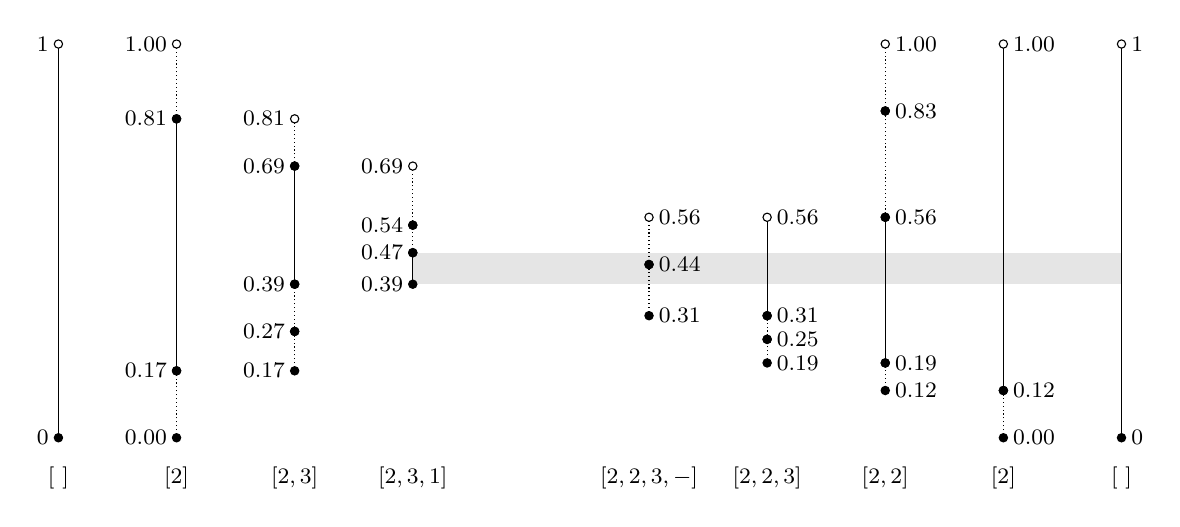
\begin{tikzpicture}[scale=0.05]
		% Final interval range
		\fill [opacity=0.1] (-30,0.39*100) rectangle (150,0.47*100);
		
		% Input side
		\intervalBothLabels{-120}{0}{100}{0}{1}{solid}{left}
		\node[below] at (-120,-5) {\footnotesize $[~]$};
	
		\intervalBottomLabel{-90}{0}{100}{0.00}{0.17}{densely dotted}{left}
		\intervalBottomLabel{-90}{0}{100}{0.17}{0.81}{solid}{left}
		\intervalBothLabels{-90}{0}{100}{0.81}{1.00}{densely dotted}{left}
		\node[below] at (-90,-5) {\footnotesize $[2]$};
	
		\intervalBottomLabel{-60}{0}{100}{0.17}{0.27}{densely dotted}{left}
		\intervalBottomLabel{-60}{0}{100}{0.27}{0.39}{densely dotted}{left}
		\intervalBottomLabel{-60}{0}{100}{0.39}{0.69}{solid}{left}
		\intervalBothLabels{-60}{0}{100}{0.69}{0.81}{densely dotted}{left}
		\node[below] at (-60,-5) {\footnotesize $[2,3]$};
	
		\intervalBottomLabel{-30}{0}{100}{0.39}{0.47}{solid}{left}
		\intervalBottomLabel{-30}{0}{100}{0.47}{0.54}{densely dotted}{left}
		\intervalBothLabels{-30}{0}{100}{0.54}{0.69}{densely dotted}{left}
		\node[below] at (-30,-5) {\footnotesize $[2,3,1]$};
		
		% Output side
		\intervalBothLabels{150}{0}{100}{0}{1}{solid}{right}
		\node[below] at (150,-5) {\footnotesize $[~]$};
	
		\intervalBottomLabel{120}{0}{100}{0.00}{0.12}{densely dotted}{right}
		\intervalBothLabels{120}{0}{100}{0.12}{1.00}{solid}{right}
		\node[below] at (120,-5) {\footnotesize $[2]$};
	
		\intervalBottomLabel{90}{0}{100}{0.12}{0.19}{densely dotted}{right}
		\intervalBottomLabel{90}{0}{100}{0.19}{0.56}{solid}{right}
		\intervalBottomLabel{90}{0}{100}{0.56}{0.83}{densely dotted}{right}
		\intervalBothLabels{90}{0}{100}{0.83}{1.00}{densely dotted}{right}
		\node[below] at (90,-5) {\footnotesize $[2,2]$};
	
		\intervalBottomLabel{60}{0}{100}{0.19}{0.25}{densely dotted}{right}
		\intervalBottomLabel{60}{0}{100}{0.25}{0.31}{densely dotted}{right}
		\intervalBothLabels{60}{0}{100}{0.31}{0.56}{solid}{right}
		\node[below] at (60,-5) {\footnotesize $[2,2,3]$};
	
		\intervalBottomLabel{30}{0}{100}{0.31}{0.44}{densely dotted}{right}
		\intervalBothLabels{30}{0}{100}{0.44}{0.56}{densely dotted}{right}
		\node[below] at (30,-5) {\footnotesize $[2,2,3,-]$};
	\end{tikzpicture}
	
	\caption{\label{fig:interval_algorithm} Example run of the interval algorithm. On the left, an input sequence $[2,3,1]$ from the source process gets mapped to $[0.39,0.47)$. On the right, this interval allows to generate up to 3 terms of an output sequence from the target process, \ie $[2,2,3]$, which corresponds to $[0.31,0.56)$. Note that it is not possible to generate more terms of the output sequence, as neither $[0.31,0.44)$ nor $[0.44,0.56)$ is a superinterval of $[0.39,0.47)$.}
	
\end{figure}

\section{Stegosystem based on the interval algorithm}
\label{sec:plain_stegosystem}

The algorithm introduced in section~\ref{sec:interval_algorithm} can be used to create a stegosystem as shown below:

\begin{figure}[h]
	\centering
	
	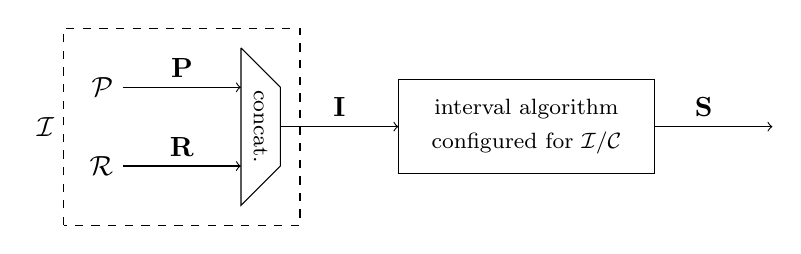
\begin{tikzpicture}[xscale=0.05,yscale=0.05]
		
		% Plaintext source P
		\node [left] at (0,10) {$\mathcal P$};
		\draw [->] (0,10) -- (30,10);
		\node [above] at (15,10) {$\mathbf P$};
		
		% Randomness source R
		\node [left] at (0,-10) {$\mathcal R$};
		\draw [->] (0,-10) -- (30,-10);
		\node [above] at (15,-10) {$\mathbf R$};
		
		% Concatenation of P and R
		\draw (30,20) -- (40,10) -- (40,-10) -- (30,-20) -- (30,20);
		\node [rotate=270] at (35,0) {\footnotesize concat.};
		
		% Process I
		\draw [dashed] (-15,-25) -- (-15,25) -- (45,25) -- (45,-25) -- (-15,-25);
		\node [left] at (-15,0) {$\mathcal I$};
		
		% Input sequence I
		\draw [->] (40,0) -- (70,0);
		\node [above] at (55,0) {$\mathbf I$};
		
		% Interval algorithm
		\draw (70,-12) -- (70,12) -- (135,12) -- (135,-12) -- (70,-12);
		\node [align=center] at (102.5,0) {\footnotesize interval algorithm \\ \footnotesize configured for $\mathcal I / \mathcal C$};
		
		% Output sequence S
		\draw [->] (135,0) -- (165,0);
		\node [above] at (147.5,0) {$\mathbf S$};
		
	\end{tikzpicture}
	
	\caption{\label{fig:stegosystem} $\mathcal P$ is the source of plaintext and $\mathcal R$ is any arbitrary stochastic process, for example a sequence of \iid bits. Both $\mathcal P$ and $\mathcal R$ have known stochastic models. $\mathcal C$ is the stochastic model of the covertext. The process $\mathcal I$ is the concatenation of the finite sequence output by $\mathcal P$ (the secret message $\mathbf P$ of length $N$) followed by the infinite output of $\mathcal R$. $\mathcal I$ is then used as input to the interval algorithm, generating an output sequence according to $\mathcal C$ -- the stegotext $\mathbf S$ of arbitrary length $M$. $M$ is chosen to be large enough so that $\mathbf P$ can be recovered in full from $\mathbf S$.}
	
\end{figure}

The stegotext sequence $\mathbf S$ is generated according to the covertext source $\mathcal C$, so the stegotext is innocuous (\ie statistically indistinguishable from covertext) by construction. However, the system does not implement any kind of key-based secrecy -- upon knowledge of the system, both the enemy and recipient can decode the plaintext secret message $\mathbf P$.

The recovery of $\mathbf P$ from $\mathbf S$ deserves more explanation. Let us denote by $\mathbf I$ the input sequence from $\mathcal I$ that was used to generate the output sequence $\mathbf S$. Let us also denote the intervals corresponding to particular sequences (according to their stochastic models) by lowercase bold serif letters, \ie $\mathbf p$ for $\mathbf P$, $\mathbf i$ for $\mathbf I$, \etc.

To generate $\mathbf S$, we need $\mathbf i \subseteq \mathbf s$. If we simply used $\mathbf P$ as $\mathbf I$, then $\mathbf p = \mathbf i$. But $\mathbf s$ as a superinterval of $\mathbf p$ would not be enough to identify $\mathbf P$. Consult Fig.~\ref{fig:interval_algorithm} and imagine that $\mathbf I = \mathbf P = [2,3,1]$. $\mathbf i = [0.39,0.47)$ would generate $\mathbf S = [2,2,3]$. However, $\mathbf s = [0.31,0.56)$ could have come from $[0.39,0.47)$ (\ie $[2,3,1]$), or $[0.47,0.54)$ (\ie $[2,3,2]$), or in fact any interval mapped from an extension of $[2,3,1]$ or $[2,3,2]$. This is why we need the process $\mathcal R$ to extend $\mathbf P$ to $\mathbf I = \mathbf P + \mathbf R$ such that the following inequality holds: $\mathbf i \subseteq \mathbf s \subseteq \mathbf p$ (\ie keep generating $\mathbf S$ using $\mathcal I$ until $\mathbf s \subseteq \mathbf p$).

This can pose another problem -- $\mathbf s$ might be \emph{too much} smaller than $\mathbf p$, \ie $\mathbf s$ may allow us to keep decoding from the model $\mathcal P$ past the actual length of $\mathbf P$. We need extra information to know when we reach the end of sequence $\mathbf P$. This can be achieved by for example storing length $N$ using universal coding at the start of $\mathbf P$, or by appending a unique EOF symbol at the end of $\mathbf P$.

\section{Stochastic process models of plaintext and covertext}

Both plaintext and covertext can be viewed as a sequence of atomic elements. The elements can be either letters or full words, extended by punctuation and special symbols such as EOF or start/end of sentence markers, in total comprising the alphabet $\mathbb E$. The interval algorithm requires the ability to evaluate the probability of $(k+1)$th element $e_i \in \mathbb E$ given the preceding sequence $\mathbf E_{kj} \in \mathbb E^k$. Taking a frequentist approach to probability, this number can be expressed by the following equation (where the $+$ operator denotes concatenation of sequences):

\begin{equation}
\label{eq:conditional_element_probability}
P(e_{i} | \mathbf E_{kj}) = \frac {\mathrm{Freq} (\mathbf E_{kj} + [ e_{i} ])} {\sum_{i'=1}^{| \mathbb E |} \mathrm{Freq} ( \mathbf E_{kj} + [e_{i'}] )}
\end{equation}

Computing Eq.~\ref{eq:conditional_element_probability} exactly is difficult because the size of the frequency table increases exponentially with the length of sequence $k$. Such a model would also easily overfit the data, even if to calculate the frequencies we used the corpus of all sentences ever written. The space complexity of the problem can be reduced by assuming that $e_i$ is independent of symbols more than $n-1$ positions before it, \ie that the sequence is generated according to an $n$th order Markov chain. Sequence substrings of length $n$ are commonly called ngrams in natural language processing literature. Eq.~\ref{eq:conditional_element_probability} can be then simplified to Eq.~\ref{eq:nth_order_conditional_element_probability}, where $\mathbf E^{(n)}_{kj}$ consists of $\min(n, |\mathbf E_{kj}|)$ last elements of $\mathbf E_{kj}$.

\begin{equation}
\label{eq:nth_order_conditional_element_probability}
P(e_{i} | \mathbf E_{kj}) \approx P(e_{i} | \mathbf E^{(n-1)}_{kj}) = \frac {\mathrm{Freq} (\mathbf E^{(n-1)}_{kj} + [ e_{i} ])} {\sum_{i'=1}^{| \mathbb E |} \mathrm{Freq} ( \mathbf E^{(n-1)}_{kj} + [e_{i'}] )}
\end{equation}

The frequency table of ngrams will be incomplete even with the above simplification -- not every sequence from $\mathbb E^n$ will be found in the corpus at least once, even for modest $n$.  As a result, either the numerator or both the numerator and denominator of Eq.~\ref{eq:nth_order_conditional_element_probability} can be 0. Both cases pose a problem since each sequence to be mapped to an interval needs to have a well-defined, non-zero probability.

If we want to be able to process any input sequence that is in $\mathbb E^k$, we can introduce a \emph{back-off} symbol to the plaintext model. If the next term in the input sequence $e_i$ has an undefined or 0 probability, we choose the subinterval corresponding to the back-off symbol and re-evaluate the probability of $e_i$ using a lower order model. Finally, a $1$st order model has to return a valid non-zero probability, or else the term would not be in the alphabet.

To keep generating the stegotext sequence, it suffices to be able to evaluate the probability of at least one term given the preceding sequence. If no terms are available, the decision to back-off the model can be made implicitly. However, in order to increase the variety of possible output sequences, it might be worth introducing a back-off symbol in the stegotext model as well.

\subsection{Sources of ngram frequencies for words and letters}

The Google Books Team has released a database of word ngram frequencies (up to $n=5$) that contains a total of 468 billion ngrams from 4.5 million English books. \cite{googlengrams2011} Ngrams include part-of-speech (POS) annotations for words and special markers for the beginning and end of a sentence. They are grouped by years and never span sentence boundaries. The cutoff for including an ngram in the database is $\ge40$ occurrences in the whole corpus.

Mark Davies has compiled databases of word ngram frequencies (up to $n=4$ and $n=5$) from the Corpus of Contemporary American English (COCA). \cite{coca2010, web:byu_ngrams} The ngrams include POS-annotated words and punctuation, but no special markers. Free version of the database contains 1 million most frequent ngrams for each $n$ up to $n=5$. Paid version contains all ngrams up to $n=4$, \ie a total of 155 million ngrams.

Freek Dijkstra has calculated single character frequencies from 120 most popular Project Gutenberg books. \cite{web:letter_distribution}

\section{Progress made}

\subsection{Implementation}

I have implemented a proof of concept system as described in section \ref{sec:plain_stegosystem}, \ie without any secrecy. I used single letter frequencies for the plaintext model, and the free COCA ngrams database for the covertext model. I used "\texttt{.}" as the EOF symbol in plaintext.

The interval algorithm and both plaintext and covertext models were implemented in Mathematica. The COCA database was processed using Python and stored in a PostgreSQL database. Single letter frequencies were stored in the source code.

\subsection{Results}

An example plaintext "\texttt{TERMINATE.}" generates the following stegotext, which successfully translates back to the same input sequence:

\begin{quote}
that he was preparing to leave for the airport and the extent of the government and the press
\end{quote}

The output sounds English, but lacks features such as start or end of a sentence or punctuation. The stegotext is long due to low plaintext compression rate (here: underestimating the probability of plaintext sequence leads to a small input interval) and low entropy of the stochastic model of covertext (a long sequence is needed to achieve small output interval).

\section{Future work}

\subsection{Secrecy}

The next most important aspect of the project is secrecy. The simplest way to address it is to use already developed cryptographic techniques. For example, compress plaintext to a sequence of bits (\eg using arithmetic coding), encipher the sequence with a secret key (\eg using a stream cipher), and finally feed in the enciphered sequence to the interval algorithm in order to generate stegotext. If the entropy of the key is higher than the entropy of plaintext, it can be proved that perfect secrecy is achieved.

A more interesting way to encipher plaintext is by doing interval arithmetic. Showing that perfect secrecy can be achieved by for instance shifting the plaintext interval by a certain number could be a novel result in the field of information theory.

After having implemented procedures for secrecy, a measure of it should be developed as well. An interesting concept of deniable encryption could also be pursued -- the system given a random key might be able to generate plausible plaintext from stegotext. Different schemes of encryption, such as public-key cryptography, can be explored as well.

\subsection{Richer ngram models}

The quality of the output can be improved if a richer ngram model is employed. The Google Books Ngrams database contains many more ngrams than the free COCA ngrams database used so far. The former should result in more varied, \ie natural, stegotext. Higher entropy of the covertext model would decrease expected length of the output sequence. Additionally, start and end of sentence markers should make it possible to produce structured sentences.

Similarly, the single letter frequency plaintext model can be replaced with a better one. One option is to scan the Project Gutenberg books database to extract higher-order letter ngram frequencies. It is also possible to process the Google Books Ngrams database to do the same thing.

\subsection{Rate of the system}

Rate of the system could be defined and investigated. Han \& Hoshi \cite{hanhoshi1997} state asymptotic bounds on the performance of the interval algorithm to generate output sequences of finite length. It might be possible to argue that performance of the stegosystem can be bounded by considering the analysis from \cite{hanhoshi1997} with the input and output reversed.

\subsection{Communicating the length of plaintext}

It is necessary to somehow communicate the length of plaintext $N$ in order to be able to correctly decode it. The difference between storing $N$ at the beginning of plaintext (or ciphertext) and appending an EOF symbol at the end of plaintext (or ciphertext) should be investigated. The two methods might result in different performance and/or security of the system.

\subsection{More advanced language models}

A sentence can be represented not only as a linear sequence of characters of words. For example, a \emph{wh-clause} (\ie one that uses pronouns such as \emph{what}, \emph{where}, \etc) can be separated by more than a few words, so it can't be adequately represented by ngrams. It is possible to use grammatical rules to parse a sentence into a tree, so that the relationship between particular words is exposed.

The problem is that the tree representation would have to be both parsed and generated in a consistent and linear manner. This is a very interesting problem in the field of algorithms and linguistics, but most likely is outside the scope of this project.

\subsection{Finite precision arithmetic coding}

Interval mapping in arithmetic coding is usually performed using finite precision arithmetic, because infinite precision arithmetic does not scale well on current hardware. In my implementation I am representing the intervals exactly using rational numbers. I have run tests that show that the algorithm can easily transform a sentence of plaintext into a paragraph of stegotext. However, it will likely not scale to input sizes in the order of a book. Finite precision interval mapping would solve this problem, but also introduce other issues such as complications due to interval rounding. The required changes to the interval algorithm and the stegosystem might be very substantial and outside the scope of the project.

\footnotesize
\bibliographystyle{unsrt}
\bibliography{../bibliography}

\end{document}
